\section{Présentation de l'\ifsttar}
  \subsection{L'établissement}

J'ai effectué mon stage à l'Institut Français des Sciences et Technologies des Transports, de l'Aménagement et des Réseaux (\ifsttar). C'est un "\glsdesc{EPST}" (\bsc{\gls{EPST}}*). Créé en 2011, il est placé sous la double tutelle du Ministère de l'Écologie, du Développement durable et de l'Énergie et du Ministère de l'Enseignement supérieur et de la Recherche.

\begin{figure}
  \centering
  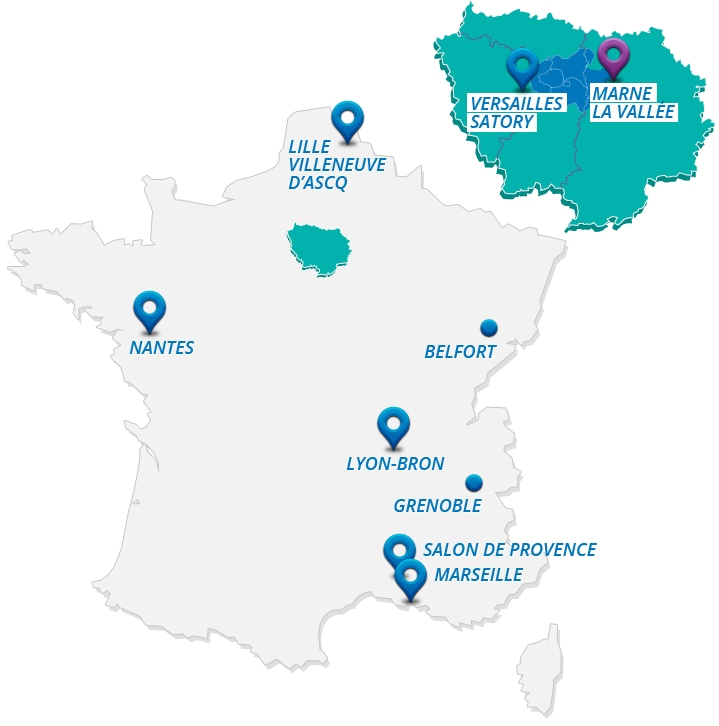
\includegraphics[height=25em]{contextualisation_du_stage/carte_sites_ifsttar}
  \caption{Répartition des différents sites de l'\ifsttar}
\end{figure}

Au total, l'\ifsttar rassemble environ un millier d'agents, dont 350 chercheurs. Il y a environ 380 doctorants accueillis dans les laboratoires de l’\ifsttar. L'\ifsttar comporte 5 départements de recherche distincts (voir annexe A). Par ailleurs, l’\ifsttar dispose d’un large patrimoine d’équipements scientifiques, qui lui permet de développer une recherche et une expertise de haut niveau. En effet, il s’agit d’équipements rares qui permettent à l’\ifsttar de conduire des travaux de recherche. Ces équipements scientifiques  sont très diversifiés : des sites et plateformes d'expérimentation, des simulateurs, des véhicules instrumentés, ou encore des recueils de données. Une importante production scientifique (thèses, publications, rapports de recherche) découle de ces équipements indispensables aux structures de recherche pour la mise en œuvre de leurs travaux.

  \subsection{Le site de Bouguenais}

\begin{figure}
  \centering
  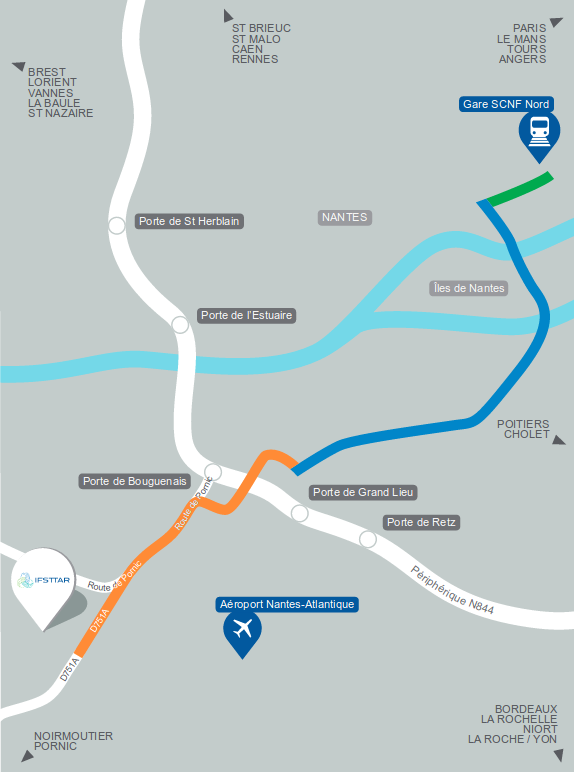
\includegraphics[height=25em]{contextualisation_du_stage/plan_acces_site_bouguenais}
  \caption{Plan d'accès du site de Bouguenais}
\end{figure}

Il y a 12 laboratoires représentant 4 départements sur le site de Bouguenais.

\begin{figure}
  \centering
  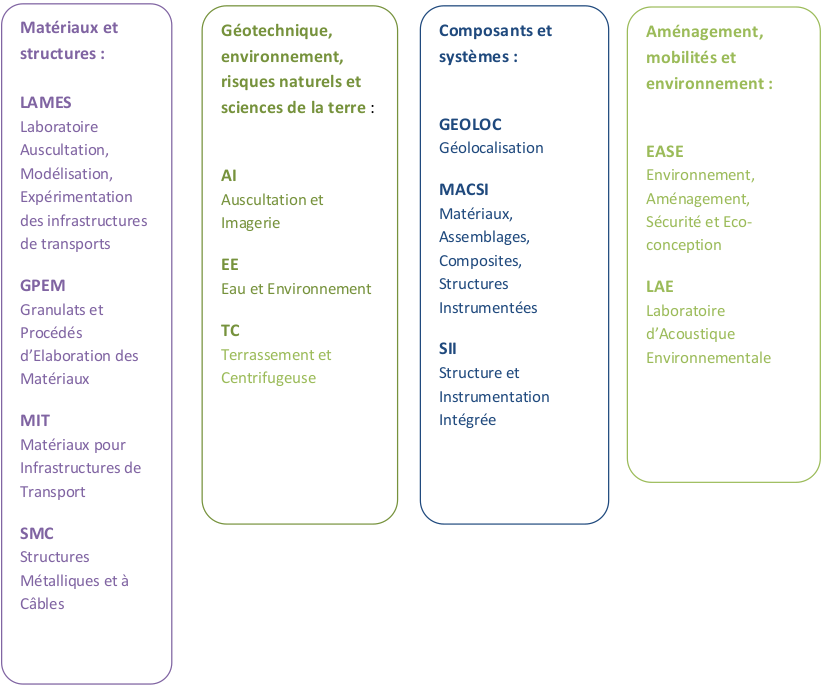
\includegraphics[height=25em]{contextualisation_du_stage/laboratoires_site_bouguenais}
  \caption{Laboratoires présents sur le site de Bouguenais}
\end{figure}


\section{Environnement et outils de travail}
  \subsection{Laboratoire d'accueil}

J'ai été accueilli au sein du laboratoire "Environnement, Aménagement, Sécurité et Eco-conception"(\bsc{EASE*}) du département "Aménagement, mobilités et environnement" (\bsc{\gls{AME}}*). Au sein du bâtiment, j'ai également été en contact avec des personnes du laboratoire (\bsc{\gls{LAMES}}*) du département "Matériaux et structures".

  \subsection{Ressources matérielles et logicielles à disposition}

J'avais bien entendu un bureau à disposition. J'avais également à disposition un tableau blanc qui m'a beaucoup servi pour les activités de conception, ainsi que pour réfléchir sur les problématiques qui ont pu se poser au long du projet.

Pour le développement, j'avais à disposition un ordinateur en dual boot, avec deux systèmes d'exploitation à ma disposition : Windows 7 et Ubuntu 16.04 \bsc{\gls{LTS}}*. Cependant je n'ai utilisé que Linux.

En ce qui concerne le déploiement de mon application, une machine nous a été rendue disponible en \gls{SSH}*. Ce serveur a notamment un disque ayant une capacité de stockage nécessaire pour traiter d'importants ensembles de données.

  \subsection{Outils utilisés}

Je me suis muni des outils avec lesquels je suis à l'aise. Ils m'ont permis de gérer et de mener à bien mon développement de manière efficace.

\begin{description}
  \item[\gls{PyCharm}*~:] \bsc{\gls{IDE}}* en version professionnelle (licence étudiante offerte par \gls{JetBrains}*)
  \item[\gls{conda}* + \gls{pip}*~:] facilitateurs de gestion des dépendances via la création d'un environnement virtuel d'exécution
  \item[\gls{git}* + \gls{GitHub}*~:] gestionnaire de version
  \item[\gls{markdown}*~:] langage à la syntaxe enfantine pour les productions rapides de petits documents
  \item[\bsc{\gls{LaTeX}}*~:] langage de présentation utilisé pour la rédaction du cahier des charges et de ce rapport
  \item[\gls{Atom}*~:] éditeur de texte, que j'ai surtout utilisé pour le markdown et le \bsc{LaTeX}
  \item[\gls{SublimeText}*~:] éditeur de texte, utilisé en complément d'Atom
\end{description}

  \subsection{Organisation et méthodologie}

L'organisation d'équipe que l'on a suivi reprend plusieurs point importants que l'on peut retrouver en méthode agile :

\begin{itemize}
  \item des évolution rapides au niveau des spécifications~;
  \item des réunions  assez courtes avec quelques questions par personne et un tableau à disposition~;
  \item une communication permanente au sein de l'équipe sur la fonctionnalité dont le développement est à prioriser~;
  \item un développement itératif~;
  \item une version fonctionnelle de l'application à tous les stades du développement~;
  \item des tests effectués sur les fonctionnalités au fur et à mesure de l'avancement.
\end{itemize}

  \subsection{Prise de notes}

Tout au long de mon stage, j'ai tenu un journal de bord qui décrit ce que j'ai réalisé au jour le jour. Par ailleurs, j'ai conservé les liens des ressources utiles que j'ai trouvées lors de mes recherches ou que l'on a pu me signaler. Je les ai accompagnés d'une description succincte indiquant la nature des informations intéressantes que l'on peut y trouver.
